\chapter{Question 2}
\label{avoiding-uri-aliases} 

\textbf {Determine if the friendship paradox holds for your Twitter account. Since Twitter is a directed graph, use ``followers'' as value you measure
(i.e., ``do your followers have more followers than you?'').\\
Generate the same graph as in question 1, and calcuate the same  mean, standard deviation, and median values.\\
For the Twitter 1.1 API to help gather this data, see:}\\
{\url{https://dev.twitter.com/docs/api/1.1/get/followers/list}}\\
\textbf{If you do not have followers on Twitter (or don't have more than 50), then use my twitter account ``phonedude\textunderscore mln''.}

Following are the steps that I have taken to solve this problem:
\begin{itemize}
\item I did not have more than 50 followers, so I randomly picked a user with the screen name `ohttic' from your followers list. He has 258 Followers and is following 1,923 people.
\item Twitter provides an API to get the list of followers. This API returns an object of followers with the profile information. `Tweepy' library is a wrapper around Twitter that makes it easier to retrieve Twitter data. I used this library to get the followers data.
\item I iterated through the list of users and retrieved the `screen\textunderscore name', `followers\textunderscore count' and `friends\textunderscore count'. I stored this information in a JSON structure and saved it into a file `userFollowerdata' . This code is listed in Listing \ref{lst:q2code1}.
\item Furthermore, I extracted the followers count from the JSON and stored it in a file `followersCount'. This code is listed in Listing \ref{lst:q2code2}
\item I calculated the mean, median and standard deviation for the followers count. This code is listed in Listing \ref{lst:q2code3}. The mean, median and standard deviation are given in Table \ref{Table:q2table1}

\begin{table}

\caption{Mean, Median and Standard Deviation of number of followers of followers}
\label{Table:q2table1}
\begin{center}
\begin{tabular}{| c | c |}
\hline
Key & Value \\ \hline

Mean & 54474.2 \\ \hline
Median & 5477.0 \\ \hline
Standard Deviation & 120893.613437 \\ \hline

\hline

\end{tabular}
\end{center}
\end{table}

\newpage
\item Figure \ref{fig:q2fig2} illustrates the ranking of `ohttic' in terms of followers count in comparison with his followers.
\begin{figure}[h!]
\begin{center}
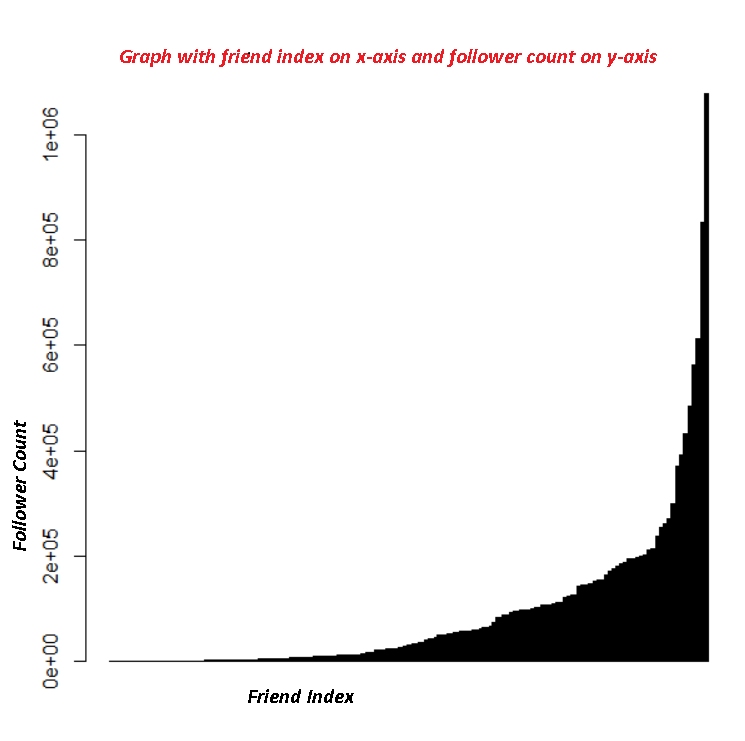
\includegraphics[scale=0.55, keepaspectratio=true]{figures/followerWithoutLog.PNG}
\caption{Graph with number of followers on y-axis and followers on x-axis }
\label{fig:q2fig2}
\end{center}
\end{figure}

\begin{figure}[h!]
\begin{center}
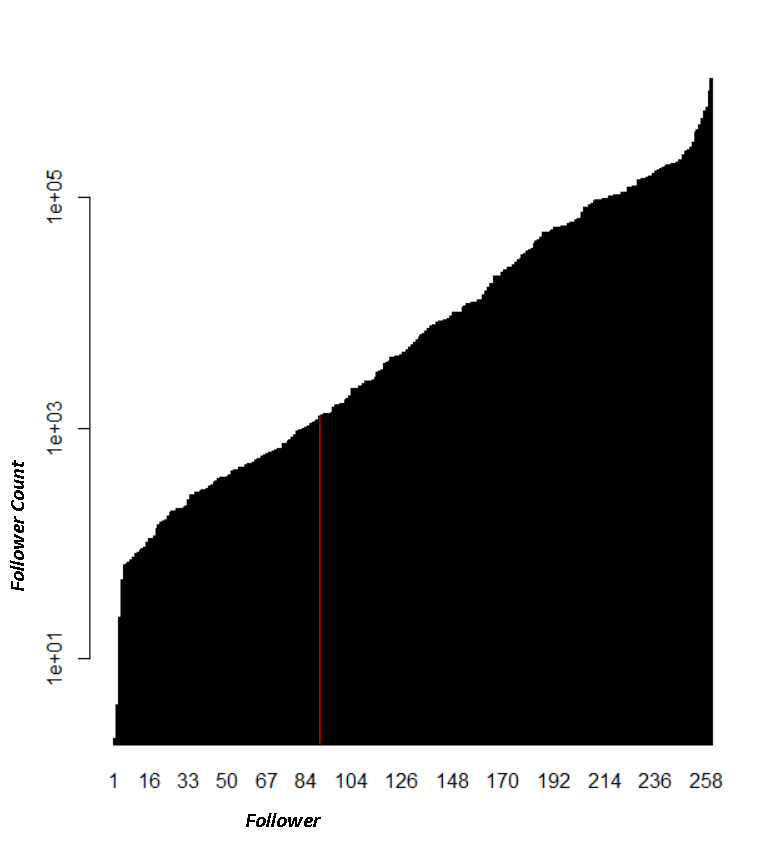
\includegraphics[scale=0.55, keepaspectratio=true]{figures/finalFollower.PNG}
\caption{Graph with number of followers on y-axis in log scale and followers on x-axis }
\label{fig:q2fig3}
\end{center}
\end{figure}
\newpage
\item From the calculated median value `5477.0' and number of followers `ohttic' have `258' we can say that he have less number of followers than his followers.

\end{itemize}

\newpage
\textbf{Code Listing}
\lstinputlisting[language=Python,caption=Python code for retrieving friends data and storing screenName followersCount and friendsCount in a JSON structure ,frame=single,label=lst:q2code1,breaklines=true,captionpos=b,numbers=left,showspaces=false,showstringspaces=false,basicstyle=\footnotesize]{src/getFollowerAndFriendsData.py}

\newpage
\textbf{Code Listing}
\lstinputlisting[language=Python,caption=Python code for extracting followers count from JSON structure,frame=single,label=lst:q2code2,breaklines=true,captionpos=b,numbers=left,showspaces=false,showstringspaces=false,basicstyle=\footnotesize]{src/extractFollowers.py}

\textbf{Code Listing}
\lstinputlisting[language=Python,caption=Python code for calculating mean median and standard deviation,frame=single,label=lst:q2code3,breaklines=true,captionpos=b,numbers=left,showspaces=false,showstringspaces=false,basicstyle=\footnotesize]{src/getMeanMedianStandardDeviation2.py}